\documentclass[conference]{IEEEtran}

\usepackage{cite}
\usepackage{graphicx}
\usepackage{booktabs}
\usepackage{array}
\usepackage{tabularx}
\usepackage{siunitx}
\usepackage{microtype}
\usepackage{url}
\usepackage{xcolor}
\usepackage{hyperref}
\usepackage{pifont}
\usepackage{balance}
\usepackage{capt-of}
\usepackage{listings}

\graphicspath{{figures/}}
\urlstyle{same}
\hypersetup{
  colorlinks=true,
  urlcolor=accentteal,
  linkcolor=accentteal,
  citecolor=accentteal,
}

\definecolor{accentteal}{HTML}{0F766E}
\definecolor{baselinegray}{HTML}{6B7280}
\definecolor{softgreen}{HTML}{2E8B57}
\definecolor{softred}{HTML}{B45309}
\definecolor{codebg}{HTML}{F5F4EF}
\definecolor{coderule}{HTML}{D6D3D1}
\definecolor{codecomment}{HTML}{78716C}
\definecolor{codetext}{HTML}{1F2937}

\setlength{\textfloatsep}{10pt plus 2pt minus 2pt}
\setlength{\floatsep}{8pt plus 2pt minus 2pt}
\setlength{\intextsep}{8pt plus 2pt minus 2pt}
\setlength{\abovecaptionskip}{4pt}
\setlength{\belowcaptionskip}{0pt}

\sisetup{
  detect-weight=true,
  table-number-alignment=center,
  group-separator={,},
}

\newcolumntype{Y}{>{\raggedright\arraybackslash}X}
\newcommand{\file}[1]{{\ttfamily\bfseries\textcolor{accentteal}{#1}}}
\newcommand{\metric}[1]{\textcolor{accentteal}{\textbf{#1}}}
\newcommand{\symnum}[1]{\textcolor{accentteal}{\textbf{#1}}}
\newcommand{\basenum}[1]{\textbf{#1}}
\newcommand{\projecturl}{\href{https://github.com/IMJONEZZ/symphonic-autoresearch}{\textcolor{accentteal}{https://github.com/IMJONEZZ/symphonic-autoresearch}}}
\newcommand{\cmark}{\textcolor{softgreen}{\ding{51}}}
\newcommand{\xmark}{\textcolor{softred}{\ding{55}}}
\newcommand{\samecore}{\textcolor{accentteal}{\textbf{preserved}}}

\lstdefinelanguage{symbash}{
  sensitive=true,
  alsoletter={-},
  morekeywords={git,cd,cp,docker,npm},
  morecomment=[l]{\#},
  morestring=[b]",
  morestring=[b]'
}

\lstdefinestyle{appendixshell}{
  language=symbash,
  basicstyle=\ttfamily\small\color{codetext},
  keywordstyle=\bfseries\color{accentteal},
  commentstyle=\itshape\color{codecomment},
  stringstyle=\color{accentteal},
  backgroundcolor=\color{codebg},
  frame=single,
  rulecolor=\color{coderule},
  framerule=0.5pt,
  framesep=6pt,
  breaklines=true,
  breakatwhitespace=false,
  columns=fullflexible,
  keepspaces=true,
  showstringspaces=false,
  tabsize=2,
  aboveskip=0.7em,
  belowskip=0.7em
}

\title{From Minimal Loop to Managed Service: A Systems Characterization of Symphonic Autoresearch}

\author{
\IEEEauthorblockN{Chris Brousseau}
\IEEEauthorblockA{Independent Researcher}
}

\makeatletter
\newcommand{\PaperFrontMatter}{
\twocolumn[
\begin{@twocolumnfalse}
\maketitle
\vspace{-1.6em}
\begin{center}
\begin{minipage}{0.96\textwidth}
\small
\textbf{Abstract}---Autonomous research loops are attractive because they can iteratively edit code, run experiments, and evaluate model quality under a fixed wall-clock budget. In practice, however, minimal loops are fragile: they are hard to restart after failure, difficult to inspect while running, and awkward to steer without tearing down the session. This paper presents a commit-pinned systems characterization of Symphonic Autoresearch as a control plane wrapped around Karpathy's minimal \file{autoresearch} loop. Auditing the 2026-03-25 and 2026-03-29 repository snapshots shows a clean contribution boundary: \file{prepare.py} is byte-for-byte identical, and \file{train.py} differs only in its top-level usage string. Symphonic therefore changes the operational envelope rather than the learning algorithm. The added system layers include workflow-configured workspace management, OpenCode session orchestration, bounded crash restart, optional stall detection, dashboard and SSE telemetry, asynchronous operator instruction delivery, and optional cross-session memory. Because the current repositories do not preserve matched raw \file{results.tsv} and \file{run.log} histories for the README comparison, this paper treats quantitative results as repository-reported context rather than reproduced evidence. The main contribution is a code-grounded account of how continuity, visibility, and steerability move from implicit operator labor into an explicit service layer around an otherwise unchanged autonomous training loop.

\vspace{0.55em}
\textbf{Index Terms}---autonomous machine learning, agentic systems, LLM training infrastructure, observability, crash recovery, experiment orchestration
\end{minipage}
\end{center}
\vspace{0.9em}
\end{@twocolumnfalse}
]
}
\makeatother

\begin{document}
\PaperFrontMatter

\section{Introduction}
Autonomous experimentation systems promise a shift from manual experiment-by-experiment iteration toward long-running search programs that continuously edit code, launch short training jobs, and decide whether to keep or discard the result. Recent agentic research systems and autonomous laboratories have pushed that idea into view across scientific discovery, software engineering, and research-assistant settings \cite{ref_automl,ref_agentlab,ref_aiscientist,ref_aiscientist_v2,ref_sweagent}. Yet building an autonomous loop is easier than building an autonomous research \emph{service}. A loop can still be fragile, opaque, and difficult to govern.

That distinction is familiar in machine learning systems more broadly. Production ML work repeatedly runs into hidden operational complexity around observability, testing, reproducibility, and technical debt \cite{ref_hidden_debt,ref_ml_test_score,ref_mlflow}. Autonomous research loops inherit those same concerns, but in a more acute form: if a long unattended run crashes, stalls, or drifts into an unproductive search region, the operator needs continuity, visibility, and steerability rather than just a terminal log.

This paper studies that transition concretely by comparing two repositories in the same workspace: Karpathy's \file{autoresearch} baseline and Symphonic Autoresearch, a TypeScript control plane that wraps the same Python experiment loop. The contribution boundary is unusually clean. At the audited commits, \file{prepare.py} is identical between repositories and \file{train.py} differs only in its usage string. Symphonic's novelty therefore lies in orchestration, recovery, telemetry, and operator control, not in a new model, optimizer, or evaluation harness.

That boundary makes the right research question clear: \emph{what changes when a minimal autonomous training loop becomes a managed service, and which of those changes are verified directly in code?} This paper answers that question through a commit-pinned repository audit rather than a matched benchmark campaign. The current repositories do not preserve the raw histories required for a fully normalized empirical comparison, so repository-reported numbers are treated as secondary context rather than the primary result.

The paper makes three contributions:
\begin{enumerate}
\item a commit-pinned audit that proves the learning core is preserved while the control plane changes;
\item a systems characterization of Symphonic's continuity, visibility, and steerability mechanisms; and
\item a methodology for separating verified code-grounded claims from repository-reported operational summaries \cite{ref_bouthillier}.
\end{enumerate}

\section{Problem Framing and Audit Methodology}
Autonomous research systems sit at an intersection between AutoML, agentic coding, and scientific workflow automation \cite{ref_automl,ref_agentlab,ref_aiscientist}. That intersection creates an interpretability problem. If a repository changes training code, prompt design, runtime supervision, deployment environment, and observability at the same time, then any improvement is hard to attribute. This paper therefore treats contribution boundaries as a first-class methodological concern.

In this repository pair, the boundary is unusually crisp. The editable research loop remains the compact Python stack inherited from \file{autoresearch}/\file{nanochat} \cite{ref_autoresearch,ref_nanochat}. Symphonic changes the surrounding conditions under which that loop operates: how the workspace is created, how failures are handled, how run state is exposed, and how a human can redirect the process.

That framing suggests four design requirements for a serious autonomous research service.

\subsection{Continuity}
A useful autonomous run must survive ordinary operational faults. Session exits, transient CLI failures, and machine restarts should reduce throughput as little as possible instead of silently terminating the overnight search budget.

\subsection{Inspectable State}
A useful autonomous run must expose enough live state for an operator to determine whether the system is progressing, spinning, or failing. In a manual workflow the operator infers that state from the terminal; in a service workflow the state should be externalized directly \cite{ref_ml_test_score}.

\subsection{Steerable Control}
A useful autonomous run should accept mid-course correction without requiring the operator to discard the whole session. This is especially important in exploratory research, where the human often notices a promising or pathological direction before the agent would.

\subsection{Auditable Artifacts}
A useful autonomous run should preserve enough artifacts to distinguish verified facts from remembered anecdotes. Reproducibility depends not just on saving code, but on preserving run conditions, result traces, and the evidence behind any claim \cite{ref_bouthillier,ref_mlflow}.

\subsection{Commit-Pinned Audit Methodology}
This paper audits two immutable snapshots: \file{autoresearch} commit \file{228791f} (full SHA: \url{228791fb499afffb54b46200aca536f79142f117}, dated 2026-03-25) and \file{symphonic-autoresearch} commit \file{130f217} (full SHA: \url{130f2172b803afd385b554f657e0d6aca23ad58a}, dated 2026-03-29). The comparison covers README and workflow prose, the vendored Python core, orchestration modules, dashboard and server code, workflow configuration, and unit tests. Claims are divided into two categories: \emph{verified code-grounded facts} and \emph{repository-reported operational summaries}. When code and prose disagree, the code is treated as authoritative for implementation claims. Quantitative statements are described as repository-reported unless the raw \file{results.tsv} or \file{run.log} histories needed to reproduce them are present.

\section{From Minimal Loop to Managed Service}
\subsection{Baseline Loop}
The baseline \file{autoresearch} repository is deliberately small. Its README identifies three files as the conceptual center of the project: \file{prepare.py}, \file{train.py}, and \file{program.md} \cite{ref_autoresearch}. The setup is designed around a fixed five-minute training budget and a single model-quality metric, validation BPB, which makes different experiments comparable even when the agent changes the architecture, optimizer, or effective model scale. The training script itself inherits from the broader \file{nanochat} lineage of compact language-model training code \cite{ref_nanochat}.

That compactness is one of the baseline's most attractive qualities. The agent's editable surface area is small, the diffs are legible, and the experiment loop is easy to explain. But that same minimalism leaves many operational concerns external to the repository. If the agent crashes, stalls, or drifts into a bad local state, the human operator is implicitly part of the recovery path. Likewise, if an overnight run is producing poor results, there is no built-in observability layer beyond terminal output.

\subsection{Contribution Boundary}
Symphonic preserves the baseline learning machinery instead of replacing it. The vendored \file{prepare.py} is byte-for-byte identical to the baseline version. The vendored \file{train.py} changes only the top-level usage comment from \file{uv run train.py} to \file{python train.py}. This matters because it prevents a common ambiguity in repository comparisons: an apparently better system can look impressive only because it quietly changed the experiment core at the same time it changed the orchestration layer.

Here, that ambiguity is minimal. The control plane is the contribution. The system's novelty lies in managing the agent, the workspace, the run state, the telemetry surface, and the intervention path around the unchanged Python experiment loop.

\begin{table}[t]
\caption{Compact audit proof for the preserved Python core}
\label{tab:core-audit}
\centering
\footnotesize
\begin{tabularx}{\columnwidth}{p{0.24\columnwidth} p{0.25\columnwidth} Y}
\toprule
File & Audit result & Why it matters \\
\midrule
\file{prepare.py} & byte-for-byte identical & Data preparation and evaluation harness are unchanged at the audited commits. \\
\file{train.py} & one-line usage-string diff only & Training logic is preserved; the visible change is operational invocation, not model code. \\
\bottomrule
\end{tabularx}
\end{table}

\subsection{Repository-Wide Comparison}
Table~\ref{tab:hero-comparison} provides the highest-level comparison. It is intentionally not just a feature checklist; it also states the systems significance of each difference, which is crucial for making the paper read like a strong systems submission rather than a changelog.

\begin{table*}[t]
\caption{High-level comparison of the baseline loop and the Symphonic control plane. The table emphasizes why each addition matters for autonomous research rather than merely listing features.}
\label{tab:hero-comparison}
\centering
\footnotesize
\begin{tabularx}{\textwidth}{p{0.16\textwidth} p{0.25\textwidth} p{0.25\textwidth} Y}
\toprule
Dimension & Autoresearch & Symphonic Autoresearch & Research significance \\
\midrule
Core experiment logic & Single-agent Python loop editing \file{train.py} under a five-minute budget & Same Python loop, copied into a managed workspace & Controls for algorithmic drift and isolates the systems contribution \\
Failure handling & Agent handles crashes inside the active terminal session & Host service detects failure and restarts with bounded backoff & Turns a fragile interactive loop into an unattended service \\
Observability & Terminal output only & Dashboard, event trace, experiment table, and hardware telemetry & Makes long runs inspectable and steerable in real time \\
Human control surface & Manual prompt edits and restarts & Asynchronous instruction injection between experiment steps & Supports corrective steering without tearing down the run \\
Deployment model & Manual local execution & Dockerized service with workflow configuration and cache mounting & Improves repeatability and operational readiness \\
\bottomrule
\end{tabularx}
\end{table*}

\section{System Overview}
Figure~\ref{fig:arch} shows the architectural boundary between the two systems. The left side is the baseline loop: one instruction file, one editable training script, and one preparation/evaluation harness. The right side is Symphonic's service layer, which is built around a TypeScript orchestrator, workspace manager, OpenCode subprocess wrapper, observability stack, and optional memory subsystem.

\begin{figure*}[t]
\centering
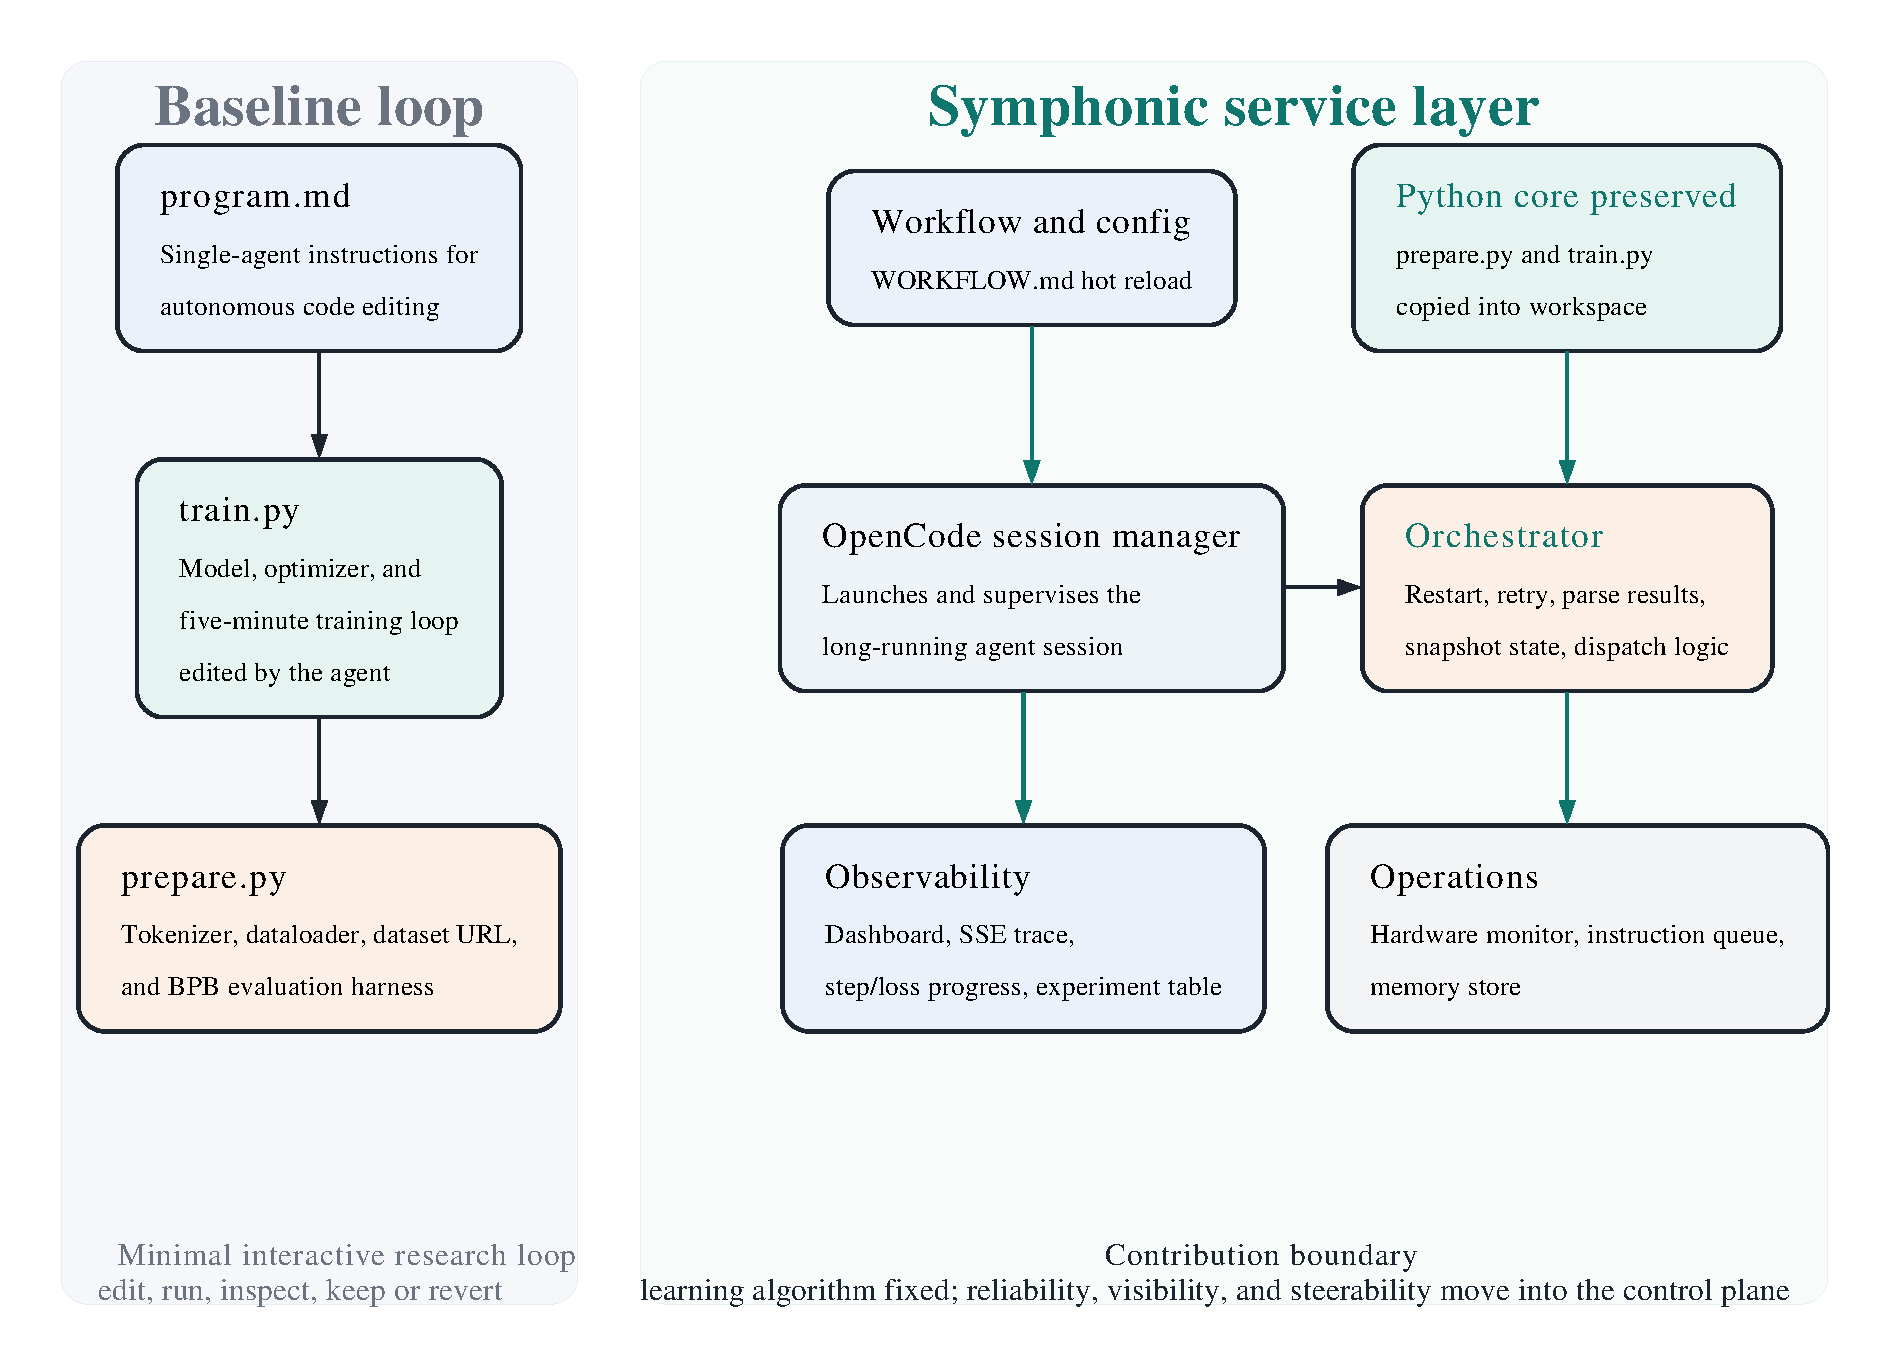
\includegraphics[width=\textwidth]{architecture_comparison}
\caption{Architecture comparison. Symphonic keeps the Python experiment core intact while moving reliability, visibility, persistence, and operator control into a separate systems layer. This separation is the paper's main contribution boundary.}
\label{fig:arch}
\end{figure*}

At startup, the Symphonic entrypoint validates GPU access, checks for the OpenCode CLI, resolves \file{WORKFLOW.md}, and launches the TypeScript service. The service builds a workspace under the configured root, copies the preserved Python files into that workspace, and invokes OpenCode with a dynamically assembled prompt and run context. The dashboard and SSE server are started alongside the orchestrator so that run state is externalized from the beginning rather than reconstructed after the fact.

The resulting lifecycle, shown in Figure~\ref{fig:lifecycle}, is what changes the research experience. A running experiment is no longer just a single agent process attached to a terminal. It becomes a managed session with explicit restart, telemetry, recovery, and intervention semantics.

\begin{figure*}[t]
\centering
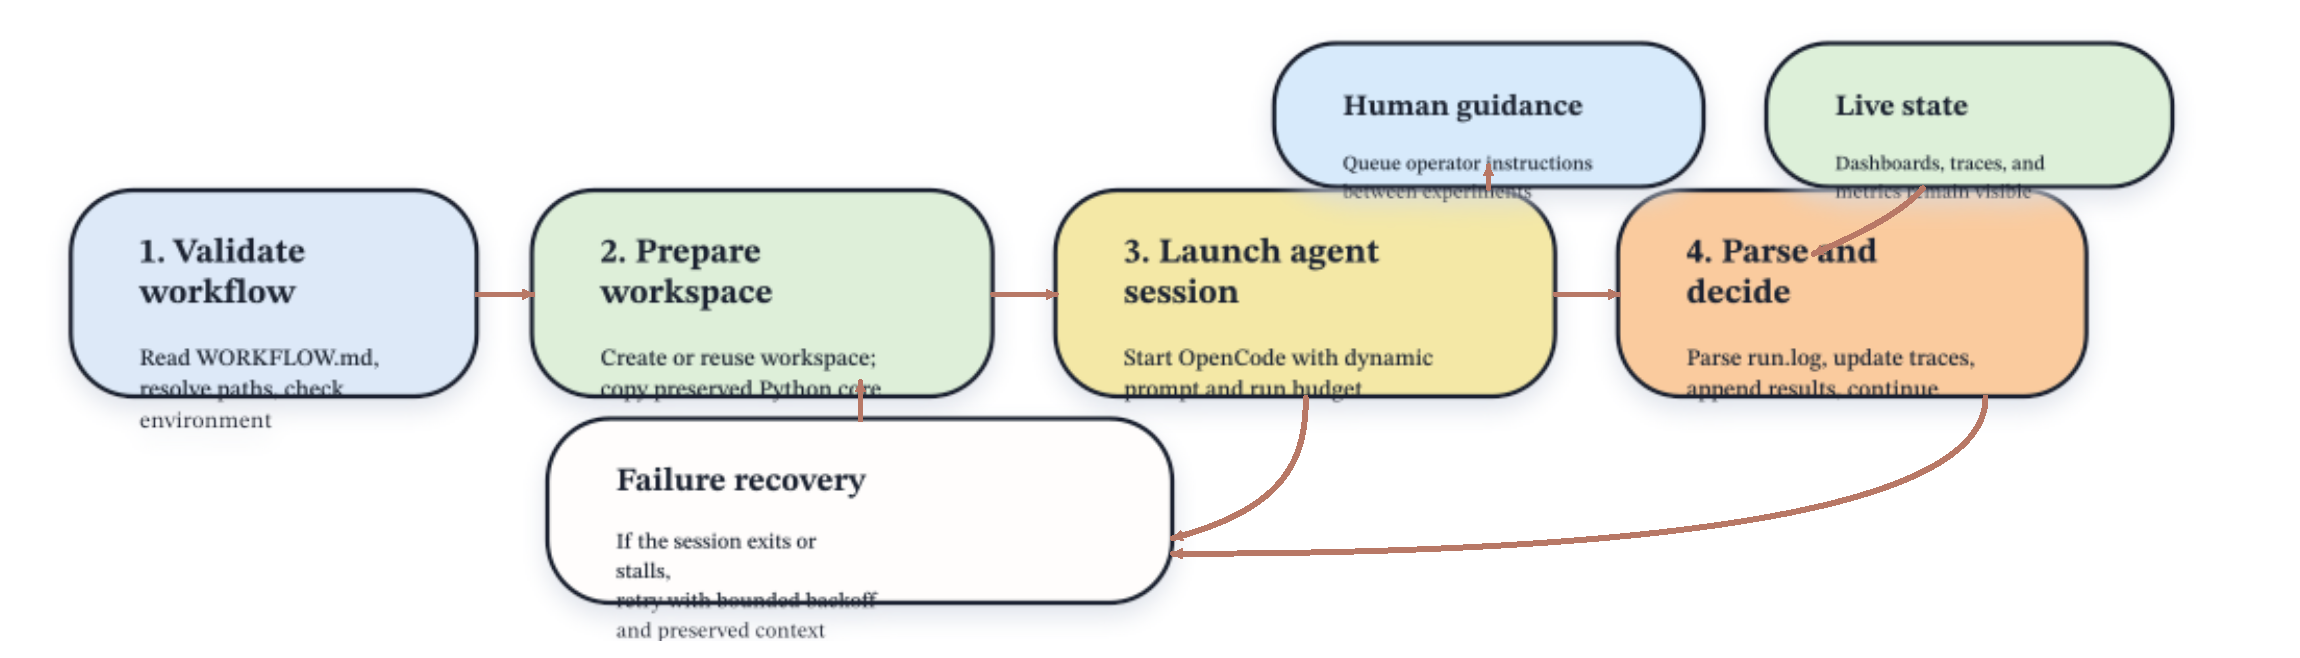
\includegraphics[width=\textwidth]{autoresearch_lifecycle}
\caption{Lifecycle of a Symphonic run. The learning loop still operates through the same Python files, but the surrounding service now owns restart, event streaming, metrics extraction, and the human intervention pathway.}
\label{fig:lifecycle}
\end{figure*}

Three design choices are especially important.

\subsection{Crash Recovery as a First-Class Systems Responsibility}
The baseline loop assumes that crashes are resolved inside an active agent session. Symphonic lifts this concern into the host service. When restart-on-crash is enabled in the workflow, an unsuccessful session exit is recorded as a crash, counted in orchestrator state, and retried with exponential backoff capped by \file{max\_retry\_backoff\_ms}. The retry queue keeps issue ownership while waiting, then reconstructs prompt context from the current workspace and prior result summaries before relaunch. Optional stall detection is controlled separately through \file{stall\_timeout\_ms}; a value of zero disables stall killing, while a positive threshold marks a run as stalled when elapsed time since last activity exceeds the configured timeout. Robustness therefore becomes an explicit property of the service rather than an informal expectation placed on the prompt.

\subsection{Observability as Part of the Product, Not an Afterthought}
Symphonic's dashboard is not merely a convenience view. The service parses \file{run.log} and result tables into step, loss, throughput, BPB, and VRAM summaries, combines them with hardware telemetry, keeps an event ring buffer for SSE streaming, and exposes those surfaces through the web UI. This means the operator can inspect not only the outcome of a run, but also its current internal state while it is in progress.

\subsection{Steerability Without Reset}
Symphonic adds a queueable instruction API that writes operator guidance into the workspace as a sidecar markdown file delivered between experiments. It also exposes an optional knowledge-persistence path gated by \file{knowledge\_enabled}. These features are operationally important, but they also matter methodologically: they make Symphonic a mixed-initiative research service rather than a pure unattended loop. The paper therefore treats instruction delivery and optional memory as verified mechanisms while remaining careful not to attribute measured gains to them without controlled ablations.

\section{Mechanisms and Hypotheses}
The reported improvement numbers in the README are interesting, but the more important scientific question is \emph{why} a systems wrapper around an unchanged training loop might plausibly improve autonomous research outcomes at all. The core claim of this section is intentionally conservative: the audited repositories verify the mechanisms, while the effect pathways remain plausible rather than conclusively proven.

\subsection{Verified Mechanisms}
Several mechanisms are visible directly in code. The service can restart failed sessions with backoff, parse run state into live dashboards, inject human guidance between steps, optionally persist embedding-backed research notes, and package the full run in a cleaner deployment environment. These are not inferred capabilities; they are implemented ones.

\subsection{Plausible Causal Pathways}
Those mechanisms suggest clear pathways to improved practical research throughput. If crash recovery prevents an unattended run from dying at 2 a.m., then the system preserves experiment continuity that would otherwise be lost. If telemetry exposes a pathological run early, then the operator can intervene sooner. If instruction injection and optional memory reduce repeated mistakes or repeated searches, then the system may spend more of its overnight budget exploring productive directions instead of re-solving the same control problem.

Crucially, these are systems explanations, not model explanations. The claim is not that observability changes the gradient update. The claim is that observability changes the likelihood that useful gradients are collected across a long sequence of unattended experiments.

\subsection{Limits of Causal Interpretation}
The current evidence base does not contain raw experiment histories, matched-hardware reruns, or time-to-best traces. Therefore, this paper does not claim that the reported 15.3\% improvement in Symphonic is caused solely by the control-plane additions. Instead, it argues that the added infrastructure addresses failure modes that are highly relevant to autonomous experimentation, and that these addressed failure modes form a credible systems explanation for why a managed service could outperform a fragile loop in practice.

Figure~\ref{fig:mechanism} summarizes this argument.

\begin{figure*}[t]
\centering
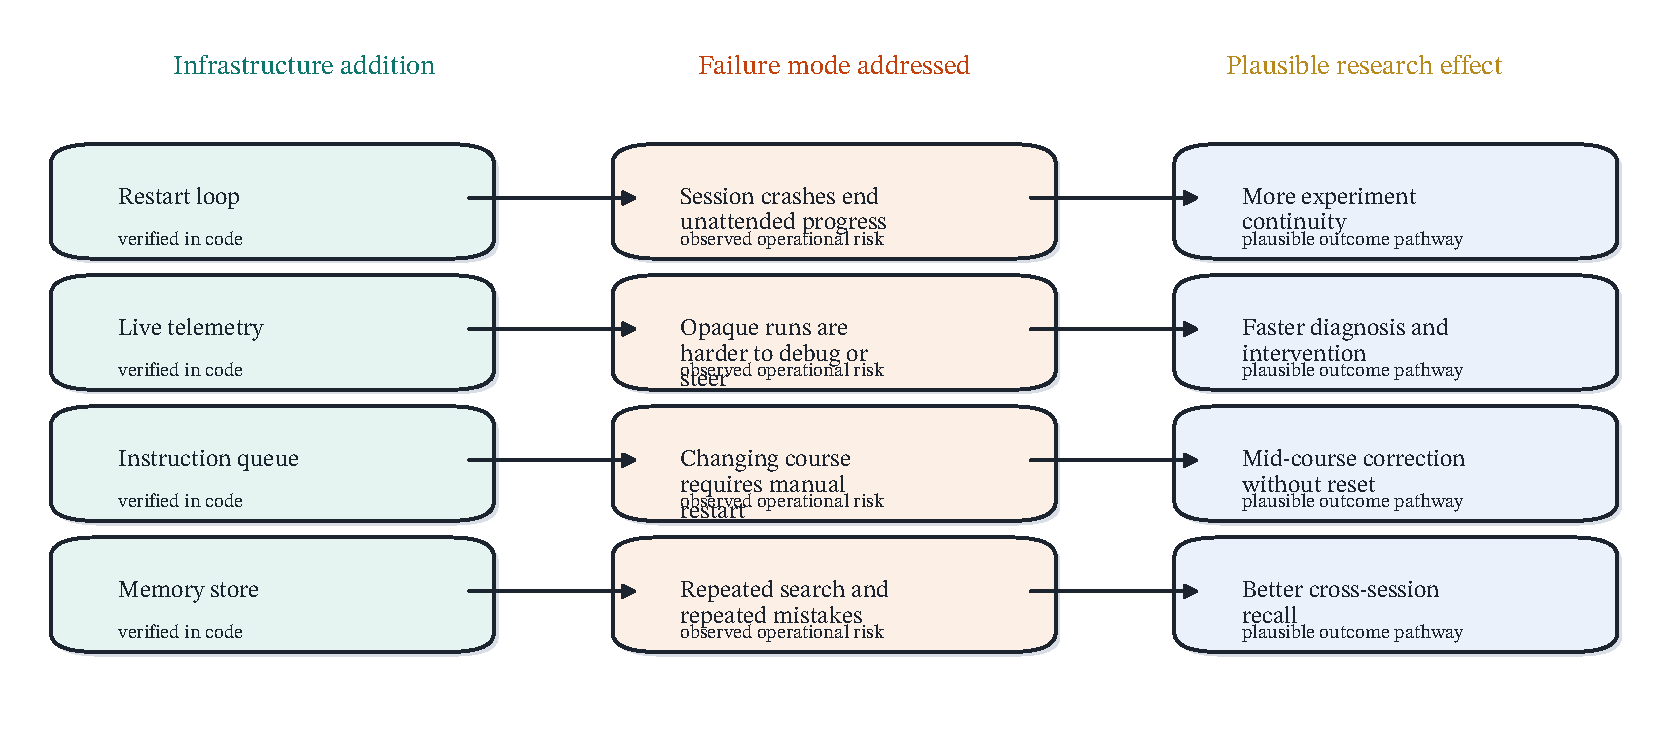
\includegraphics[width=\textwidth]{mechanism_map}
\caption{Mechanism map used in the paper's conservative causal argument. The left column is verified from code, the middle column names the operational risk being addressed, and the right column states the plausible research effect without overstating empirical certainty.}
\label{fig:mechanism}
\end{figure*}

\section{Code-Grounded Operational Comparison}
The strongest evidence in this paper is operational rather than numerical. The audited repositories show that Symphonic converts a minimal autonomous training loop into a persistent service without changing the learning core. They also show that the added value is not abstract: it is visible in restart machinery, dashboard surfaces, event streaming, instruction delivery, and workflow-driven service configuration.

\subsection{Live Observability and Control Surfaces}
Table~\ref{tab:telemetry} summarizes the live observability gap visible in the codebases themselves. The baseline loop exposes terminal summaries and post-hoc artifacts, while Symphonic adds a persistent operator surface with tracked experiments, live traces, machine telemetry, and an instruction channel. That distinction matters because autonomous experimentation becomes much easier to study once the service externalizes state that would otherwise remain trapped inside a terminal session.

\begin{table*}[t]
\caption{Observability and control surface derived directly from the codebase. This presentation is intentionally binary and readable: Symphonic's contribution is a visibly broader control surface, not a marginal visual difference on a scatter plot.}
\label{tab:telemetry}
\centering
\footnotesize
\renewcommand{\arraystretch}{1.12}
\begin{tabularx}{\textwidth}{p{0.31\textwidth} c c Y}
\toprule
Capability & Autoresearch & Symphonic & Why it matters operationally \\
\midrule
Terminal summary output & \cmark & \cmark & Both systems expose a terminal loop, so this is the shared floor rather than the differentiator. \\
Tracked experiment table & \xmark & \cmark & Gives the operator durable, glanceable run history instead of requiring manual terminal reconstruction. \\
Live step/loss trace & \xmark & \cmark & Makes it possible to see whether the current run is progressing or stalling before it ends. \\
VRAM parsing & \xmark & \cmark & Surfaces model-memory behavior that otherwise stays buried in logs. \\
GPU utilization & \xmark & \cmark & Supports operational diagnosis of under-utilization and hardware bottlenecks. \\
GPU temperature and power & \xmark & \cmark & Extends the run view from model metrics to machine-state observability. \\
System RAM visibility & \xmark & \cmark & Helps explain instability that is external to the Python training loop itself. \\
Agent event trace & \xmark & \cmark & Gives a searchable explanation surface for what the agent actually did. \\
Async instruction channel & \xmark & \cmark & Enables mid-course correction without killing and restarting the whole session. \\
\bottomrule
\end{tabularx}
\end{table*}

\subsection{Repository-Reported Snapshot}
The Symphonic README also reports a comparison between a baseline H100 run and a DGX Spark Symphonic run. Those numbers are included in Table~\ref{tab:bench} only as contextual repository-reported summaries. They are not the paper's main evidentiary backbone, because the repositories do not preserve the matched raw traces needed to reproduce or normalize them.

\begin{table*}[t]
\caption{Repository-reported comparative snapshot included for context, not as a reproduced benchmark.}
\label{tab:bench}
\centering
\footnotesize
\renewcommand{\arraystretch}{1.08}
\begin{tabularx}{\textwidth}{p{0.23\textwidth} p{0.12\textwidth} c c p{0.12\textwidth} c c c}
\toprule
System & Hardware & {Experiments} & {Kept} & {Crash status} & {Baseline BPB} & {Best BPB} & {Improvement (\%)} \\
\midrule
Karpathy autoresearch & H100 & \basenum{126} & \basenum{23} & not reported & \basenum{0.9979} & \basenum{0.9697} & \basenum{2.8} \\
Symphonic Autoresearch & DGX Spark & \symnum{52} & \symnum{22} & \textcolor{accentteal}{1 recovered} & \symnum{1.3944} & \symnum{1.1818} & \symnum{15.3} \\
\bottomrule
\end{tabularx}
\vspace{0.25em}

\raggedright\scriptsize\emph{Evidence note:} These rows come from README-reported summaries rather than preserved local run traces. Hardware, starting points, and operational conditions are not normalized, and the raw \file{results.tsv} / \file{run.log} histories needed for reproduction are not present in the audited repositories. The table is therefore interpretive context, not benchmark-grade proof.
\end{table*}

The narrower conclusion is the important one. The repository evidence is consistent with a service that sustained many experiments, counted at least one crash-and-recovery event, and externalized enough run state to make long unattended experimentation inspectable. That is already a meaningful systems result even without a matched benchmark campaign.

\section{Limitations, Reproducibility Gaps, and Future Work}
This manuscript is intentionally conservative where many repository-to-paper transitions become overconfident.

First, the contribution is not a new training algorithm. The optimizer, model architecture, evaluation harness, and fixed five-minute budget all come from the baseline loop. Symphonic contributes orchestration, operational tooling, and service semantics around that loop.

Second, the benchmark evidence is incomplete in the audited repositories. There are no raw \file{results.tsv} or \file{run.log} files for the README comparison, so we cannot independently verify per-experiment trajectories, crash categories, time-to-best curves, or restart-adjusted throughput. The quantitative material in this draft is therefore labeled as repository-reported rather than reproduced.

Third, the checked-in prose is not perfectly self-consistent. FineWeb-Edu appears in comments and configuration prose, but the checked-in data URL in \file{prepare.py} points elsewhere. This is exactly why the paper privileges code-grounded claims over prose-grounded ones.

Fourth, Symphonic is not purely autonomous in the narrowest sense. It includes asynchronous instruction delivery and optional cross-session memory, so a future controlled evaluation should report whether guidance and memory were enabled and ablate them separately from crash recovery and telemetry.

\subsection{Normalized Reproduction Campaigns}
The most immediate next step is a fresh benchmark campaign with archived \file{results.tsv}, \file{run.log}, prompt settings, workflow configuration, and environment metadata for both systems. That would replace README endpoint summaries with full traces, time-normalized comparisons, and commit-pinned reports.

\subsection{Richer Causal Telemetry}
To support stronger causal claims, the next version should record restart events, downtime between experiments, intervention timestamps, and richer metadata about why an experiment was kept or discarded.

\subsection{Multi-Agent and Hierarchical Research Orchestration}
Symphonic already shows the value of a robust control plane around a single loop. A natural extension is hierarchical or multi-agent orchestration, where planner, evaluator, retriever, and implementer agents share a coordinated workspace and telemetry surface.

\subsection{Benchmark Suites for Autonomous Research Infrastructure}
More broadly, the field needs benchmark suites that evaluate autonomous research infrastructure itself: continuity under crash, observability quality, artifact retention, steerability, intervention latency, and reproducibility. Those are systems metrics, but they increasingly determine whether autonomous experimentation can be studied rigorously at all \cite{ref_hidden_debt,ref_ml_test_score,ref_bouthillier}.

\balance
\section{Conclusion}
Symphonic Autoresearch shows that the difference between an autonomous training demo and an autonomous research service is primarily infrastructural. At the audited commits, the Python experiment core is preserved while the surrounding control plane adds restart safety, workflow-configured workspaces, live telemetry, operator intervention, and optional memory. That is the paper's verified result.

The broader implication is that autonomous research quality is increasingly a systems question. Progress will depend not only on stronger models, but also on whether the surrounding service can preserve state, recover from failure, expose evidence, accept guidance, and retain artifacts well enough to support scientific scrutiny. Symphonic makes that transition visible. It shows how a minimal autonomous loop can become a more durable, inspectable, and governable research system, even before a full matched benchmark campaign exists.

\clearpage
\onecolumn
\appendices
\section{Repository Walkthrough, Screenshot, and Adoption Notes}
This appendix is included to make the repository easier to evaluate and easier to run. The public project root is \projecturl, and the dashboard screenshot discussed here is checked into the repository at \href{https://github.com/IMJONEZZ/symphonic-autoresearch/blob/main/docs/dashboard.png}{\textcolor{accentteal}{docs/dashboard.png}}. The local copy used in this paper was taken directly from the repository's \file{docs/dashboard.png} asset.

\subsection{What the Screenshot Shows}
Figure~\ref{fig:appendix-dashboard} shows the operator-facing dashboard that differentiates Symphonic from a terminal-only autonomous loop. The top row reports session uptime, agent steps, tool calls, crash count, experiment count, and best observed validation BPB. The center of the view combines an event trace with an experiment-frontier plot, while the lower table shows per-experiment outcomes including commit identifier, validation BPB, loss, VRAM, status, and a short natural-language description of the attempted change.

This image is useful in the paper because it makes the systems contribution concrete. The screenshot is not merely promotional UI. It visually demonstrates that Symphonic externalizes the exact state that long-running autonomous experimentation otherwise keeps hidden in a terminal session: frontier progress, operator-visible failure state, hardware footprint, and a mid-run intervention surface.

\begin{center}
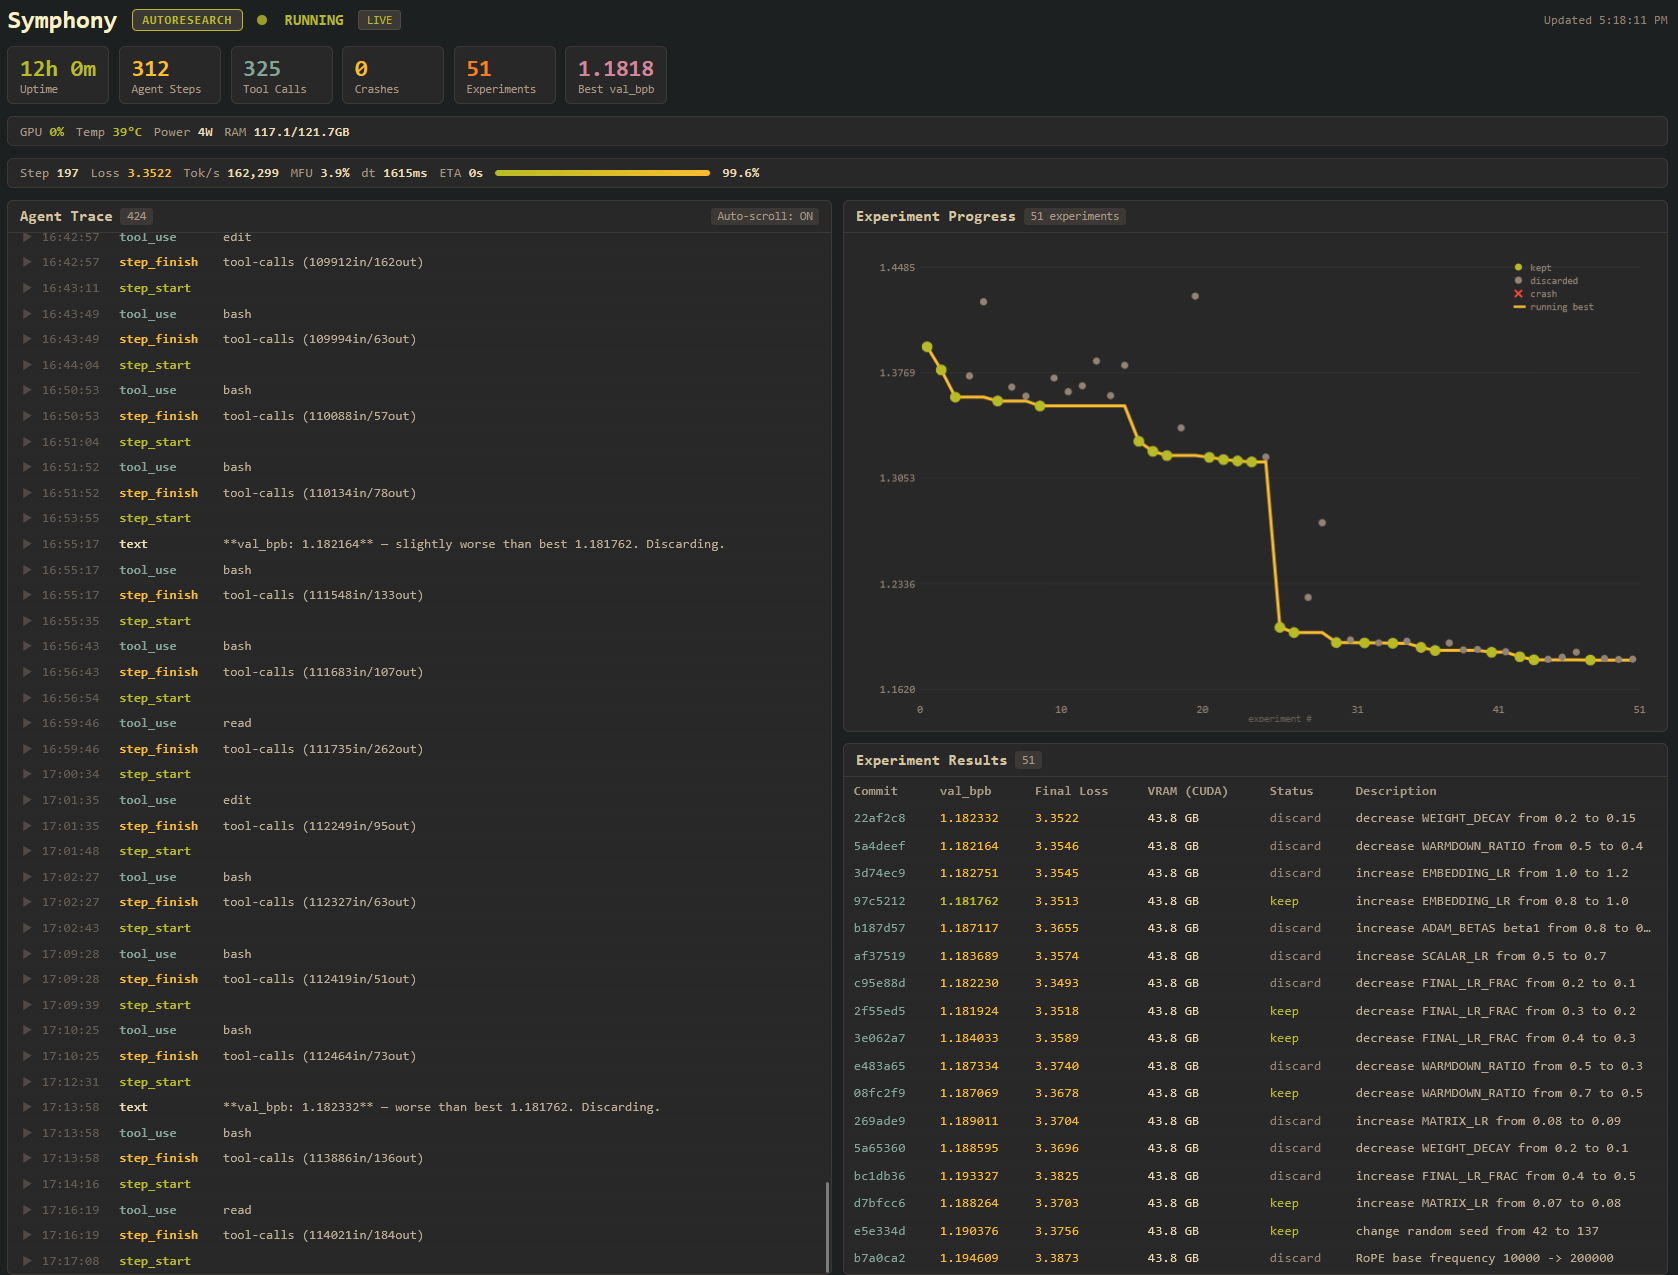
\includegraphics[width=0.92\textwidth]{dashboard_screenshot.png}
\captionof{figure}{Dashboard screenshot checked into the Symphonic repository at \file{docs/dashboard.png}. The figure shows the live operator view that turns the underlying autonomous loop into an inspectable service.}
\label{fig:appendix-dashboard}
\end{center}

\subsection{Repository Layout and Major Components}
The checked-in repository is organized to support both immediate use and extension. The \file{src/} tree contains the TypeScript service modules for orchestration, agent integration, dashboard serving, monitoring, configuration parsing, prompting, and optional knowledge persistence. The vendored \file{autoresearch/} directory contains the preserved Python experiment loop. The root-level \file{Dockerfile}, \file{docker-compose.yml}, and \file{entrypoint.sh} provide the operational path from source checkout to a running service, while \file{example.WORKFLOW.md} supplies the main user-facing configuration template.

That layout is encouraging for prospective users because it separates the stable experiment core from the service layer around it. Someone who wants to understand the training loop can stay inside \file{autoresearch/}. Someone who wants to operate the full system can follow the containerized path without first reverse-engineering the orchestration code.

\subsection{Dependencies and Runtime Expectations}
The dependency picture is also relatively approachable. The TypeScript service depends on a compact set of runtime libraries listed in \file{package.json}: \file{commander} for CLI handling, \file{express} for the dashboard server, \file{pino} for structured logging, \file{liquidjs} for prompt templating, \file{chokidar} for file watching, \file{yaml} for configuration parsing, and \file{usearch} for the optional vector-backed memory feature. Development tooling is similarly conventional: \file{typescript}, \file{tsx}, and \file{vitest}.

The container image fills in the rest of the runtime stack. The checked-in \file{Dockerfile} starts from NVIDIA's PyTorch container, installs Node.js 22, Git, and the Python packages needed by the autoresearch core, including \file{numpy}, \file{pandas}, \file{matplotlib}, \file{requests}, \file{tiktoken}, and \file{rustbpe}. The entrypoint then verifies GPU access, checks for the OpenCode CLI, runs \file{prepare.py} if the autoresearch cache is missing, and finally launches the service on port 8080.

For a new user, the practical takeaway is positive: the project has meaningful hardware and tool prerequisites, but those prerequisites are explicit rather than hidden. If a user has an NVIDIA-capable Docker setup and a configured OpenCode installation, the rest of the path is straightforward.

\subsection{License and Reuse Posture}
The repository's \file{LICENSE} file is permissive in many respects, but it is not a standard OSI permissive license. It grants broad rights to use, copy, modify, merge, publish, distribute, sublicense, and sell the software, while also adding a revenue-sharing clause that requests \metric{10\%} of gross revenue received from using the software or outputs derived from it. The summary in the checked-in license describes the project as free for personal, research, and non-commercial use, and it recommends contacting the copyright holder for commercial licensing arrangements.

That nuance is important to state clearly in the paper. Readers should feel encouraged to study and run the project, but they should also understand that commercial deployment involves terms beyond a standard MIT or Apache-style grant.

\subsection{Example Commands for New Users}
The repository already contains a practical path to first use. The command sequence below follows the checked-in README and is a good starting point for readers who want to try the system on their own hardware.

\begin{lstlisting}[style=appendixshell]
git clone \
  https://github.com/IMJONEZZ/symphonic-autoresearch.git
cd symphonic-autoresearch
cp example.WORKFLOW.md WORKFLOW.md
# Edit WORKFLOW.md with your model and preferences
docker compose up --build
\end{lstlisting}

Readers who want to verify the GPU runtime first can use the same smoke test recommended in the repository:

\begin{lstlisting}[style=appendixshell]
docker run --rm --gpus all nvidia/cuda:12-base nvidia-smi
\end{lstlisting}

And readers who prefer to inspect or develop the TypeScript service directly can use the checked-in package scripts:

\begin{lstlisting}[style=appendixshell]
npm install
npm run build
npm test
npm run dev
\end{lstlisting}

Taken together, these examples make the project approachable. The system is ambitious, but it is not mysterious: the repo exposes a direct containerized path for operators, a conventional Node/TypeScript path for developers, and a visible dashboard that rewards first-time setup with immediate feedback. Those are exactly the traits that make a research infrastructure project easier to adopt, study, and extend.

\balance
\begin{thebibliography}{99}

\bibitem{ref_symphonic}
C. Brousseau \emph{et al.}, ``Symphonic Autoresearch,'' GitHub repository, 2026. [Online]. Available: \url{https://github.com/IMJONEZZ/symphonic-autoresearch}

\bibitem{ref_autoresearch}
A. Karpathy, ``autoresearch,'' GitHub repository, 2026. [Online]. Available: \url{https://github.com/karpathy/autoresearch}

\bibitem{ref_nanochat}
A. Karpathy, ``nanochat,'' GitHub repository, 2026. [Online]. Available: \url{https://github.com/karpathy/nanochat}

\bibitem{ref_automl}
X. He, K. Zhao, and X. Chu, ``AutoML: A Survey of the State-of-the-Art,'' \emph{Knowledge-Based Systems}, vol. 212, 2021. [Online]. Available: \url{https://arxiv.org/abs/1908.00709}

\bibitem{ref_hidden_debt}
D. Sculley, G. Holt, D. Golovin, E. Davydov, T. Phillips, D. Ebner, V. Chaudhary, M. Young, J.-F. Crespo, and D. Dennison, ``Hidden Technical Debt in Machine Learning Systems,'' in \emph{Advances in Neural Information Processing Systems 28}, 2015. [Online]. Available: \url{https://papers.nips.cc/paper_files/paper/2015/hash/86df7dcfd896fcaf2674f757a2463eba-Abstract.html}

\bibitem{ref_ml_test_score}
E. Breck, S. Cai, E. Nielsen, M. Salib, and D. Sculley, ``The ML Test Score: A Rubric for ML Production Readiness and Technical Debt Reduction,'' in \emph{Proc. IEEE International Conference on Big Data}, 2017. [Online]. Available: \url{https://research.google/pubs/pub46555/}

\bibitem{ref_mlflow}
M. Zaharia, A. Chen, A. Davidson, A. Ghodsi, S. A. Hong, A. Konwinski, S. Murching, T. Nykodym, P. Ogilvie, F. Parkhe, M. Xie, and C. Zumar, ``Accelerating the Machine Learning Lifecycle with MLflow,'' \emph{IEEE Data Engineering Bulletin}, vol. 41, no. 4, pp. 39--45, 2018. [Online]. Available: \url{https://cs.stanford.edu/~matei/papers/2018/debull_mlflow.pdf}

\bibitem{ref_bouthillier}
X. Bouthillier, C. Laurent, and P. Vincent, ``Unreproducible Research is Reproducible,'' in \emph{Proc. 36th International Conference on Machine Learning}, vol. 97, pp. 725--734, 2019. [Online]. Available: \url{https://proceedings.mlr.press/v97/bouthillier19a.html}

\bibitem{ref_sweagent}
J. Yang, C. Jimenez, A. Wettig, K. Lieret, S. Yao, K. Narasimhan, and O. Press, ``SWE-agent: Agent-Computer Interfaces Enable Automated Software Engineering,'' 2024. [Online]. Available: \url{https://arxiv.org/abs/2405.15793}

\bibitem{ref_agentlab}
S. Schmidgall, Y. Su, Z. Wang, X. Sun, J. Wu, X. Yu, J. Liu, Z. Liu, and E. Barsoum, ``Agent Laboratory: Using LLM Agents as Research Assistants,'' 2025. [Online]. Available: \url{https://arxiv.org/abs/2501.04227}

\bibitem{ref_aiscientist}
R. T. Lange, Y. Lu, C. Lu, S. Hu, C. Wang, J. Foerster, J. Clune, and D. Ha, ``The AI Scientist: Towards Fully Automated Open-Ended Scientific Discovery,'' 2024. [Online]. Available: \url{https://arxiv.org/abs/2408.06292}

\bibitem{ref_aiscientist_v2}
Y. Yamada, R. T. Lange, C. Lu, S. Hu, C. Lu, J. Foerster, J. Clune, and D. Ha, ``The AI Scientist-v2: Workshop-Level Automated Scientific Discovery via Agentic Tree Search,'' 2025. [Online]. Available: \url{https://arxiv.org/abs/2504.08066}

\bibitem{ref_opencode}
OpenCode, ``OpenCode,'' software documentation, 2026. [Online]. Available: \url{https://opencode.ai}

\end{thebibliography}

\end{document}
